\section{Kinematic Features}
Kinematic data structures in DART are designed to be comprehensive, extensible, and efficient for dynamic computation. Our design principles are heavily influenced by practical use cases suggested by researchers and practitioners in Robotics. We also follow the guidelines proposed by OSRF to make DART compatible with Gazebo standard.

\subsection{Skeleton, BodyNode, and Joint}
\begin{figure*}
\centering
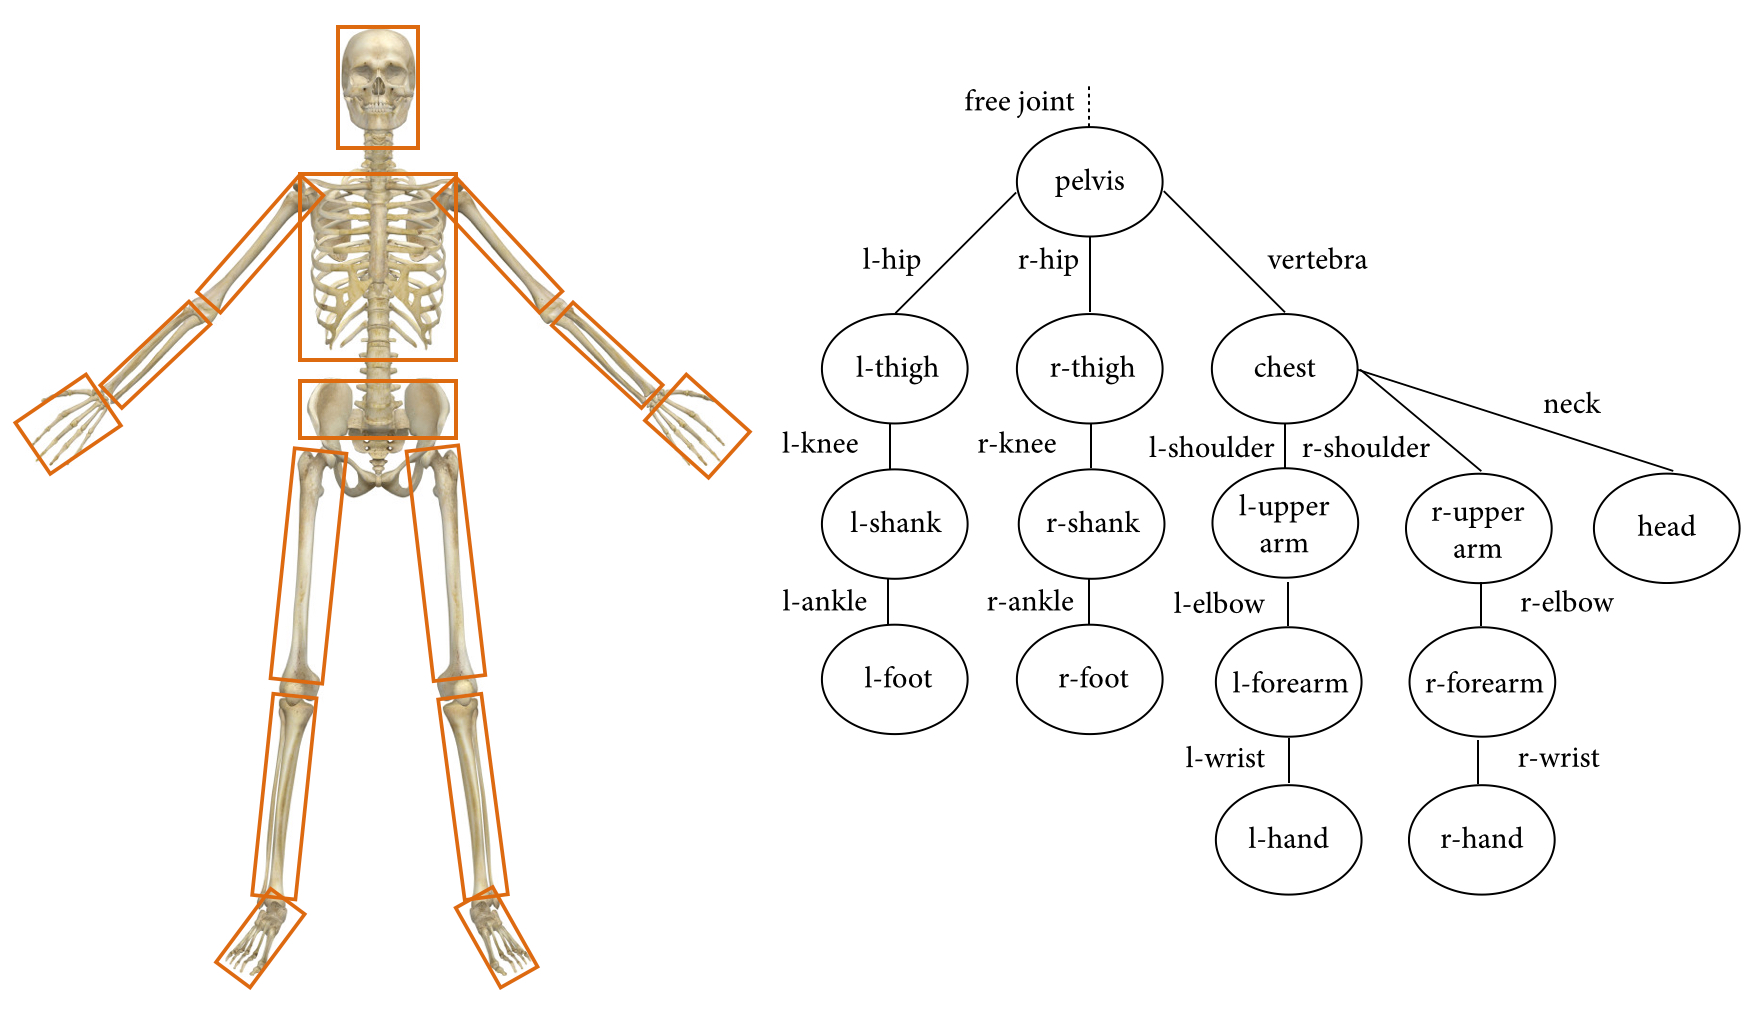
\includegraphics[width=6.0in]{fig/skeletonTree.jpg}
\caption{Tasks for each research aim.}
\label{fig:skeleton}
\end{figure*}
 In DART, an articulated dynamics model is represented by a \textbf{Skeleton}. A Skeleton is a tree structure that consists of \textbf{BodyNode}s which are connected by \textbf{Joint}s. Every Joint has a child BodyNode, and every BodyNode has a parent Joint. Even the root BodyNode has a Joint that attaches it to the \textbf{World}. For example, the human skeleton can be organized into a tree structure (Figure \ref{fig:skeleton}) with nodes representing BodyNodes and edges representing Joints. Depending on the joint type (Section \ref{sec:jointTypes}), each joint has a specific number of degrees of freedom (DOFs). For example, the hip joint can be modeled by an \textbf{EulerJoint} with three DOFs, while a knee joint can be modeled by a \textbf{RevoluteJoint} with one DOF. In this model, we select the pelvis to be the root BodyNode, which connects to the World via a \textbf{FreeJoint} with six DOFs.

A kinematic chain is a sequence of transformations from one BodyNode to another in the Skeleton. Figure \ref{fig:parentChild}(a) illustrates the transformations between two intermediate BodyNodes denoted as Parent and Child. The coordinate frames of Parent, Child, and the joint between them are shown as the RGB arrows. Let $\vc{T}_{pj}$ be the transformation from the Parent frame to the joint frame and $\vc{T}_{cj}$ be the transformation from the Child frame to the joint frame. These two transformations are fixed and can be customized as part of the \textbf{Joint::Properties} of the joint. The transformation of the joint $\vc{T}(\vc{q})$ is a function of the DOFs, $\vc{q}$, associated with the joint. In the case of the hip joint, $\vc{q}$ is a 3x1 vector consisting of hip rotation angles in three dimensions. Thus, the transformation from the Parent frame to the Child frame is denoted by $\vc{T}_{pj}\vc{T}(\vc{q})\vc{T}_{cj}^T$.

\begin{figure*}
\centering
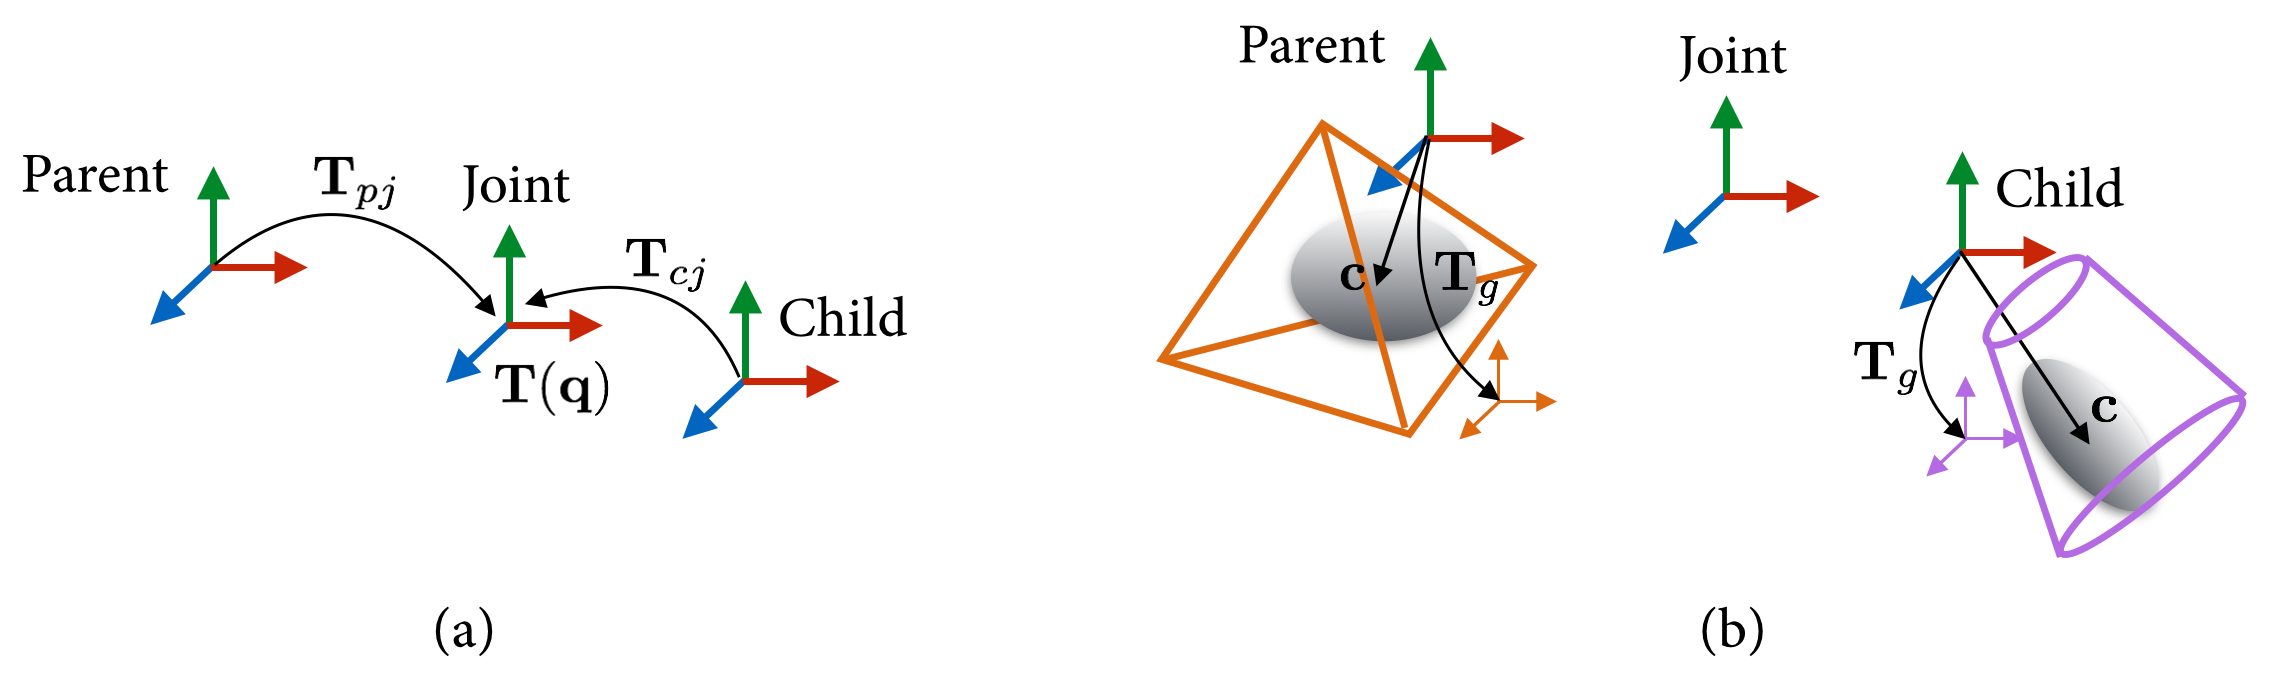
\includegraphics[width=6.0in]{fig/parentChild.jpg}
\caption{Tasks for each research aim.}
\label{fig:parentChild}
\end{figure*}


\subsection{BodyNode Properties}
A BodyNode contains a set of customizable \textbf{BodyNode::Properties} to define its kinematic and dynamic behaviors.
\begin{itemize}[leftmargin=*] \itemsep1pt \parskip0pt \parsep0pt
  \item{\textbf{Inertial properties:}} The user can define the mass, the position of the center of mass in the BodyNode frame, and the moment of inertia around the center of mass in the BodyNode frame. The ellipsoids in Figure \ref{fig:parentChild}(b) illustrate the center of mass ($\vc{c}$) and the moment of inertia defined in the BodyNode frame.
  
\todo[MXG]{We should probably mention ShapeNode when discussing geometry}

  \item{\textbf{Geometry properties:}} The user can associate a set of \textbf{Shape}s with a BodyNode. Each shape has its own geometry information used by rendering and collision detection routines. DART supports a few primitive shapes, box, ellipsoid, cylinder, plane, line segment, in addition to arbitrary 3D polygons. Each shape can be defined in its own coordinate frame. The spatial relation between the Shape and its associated BodyNode is defined by a fixed transformation $\vc{T}_g$ (Figure \ref{fig:parentChild}(b)).
  \item{\textbf{Collision properties:}} The user can set the friction coefficient and the coefficient of restitution of a BodyNode, as well as the flag that determines whether the BodyNode is collidable.
\end{itemize}

\subsection{Joint types}
\label{sec:jointTypes}
DART supports 10 types of joints. Each joint type has a fixed number of DOFs and a specific configuration domain. Some joint types require the user to define their \textbf{UniqueProperties}. For example, the rotation axes of \textbf{RevoluteJoint}, \textbf{UniversalJoint} and \textbf{PlanarJoint} need to be specified when the joint is constructed. Likewise, the order of three axes (`xyz', `zyx', etc) in an \textbf{EulerJoint} needs to be predefined. These properties can be changed at any time, and the kinematics and dynamics calculations will automatically adjust to account for those changes. The only potential negative impact would be non-physical discontinuities if property changes are made during a simulation. Note that both \textbf{BallJoint} and \textbf{EulerJoint} are used to represent rotational motion in 3D space. However, a \textbf{BallJoint} is represented by an exponential map while an \textbf{EulerJoint} is represented by three consecutive 1D rotational matrices. All joint types provided by DART are listed in Table \ref{tab:jointTypes}.

\begin{table}[h]
\centering
\caption{Joint Types}
\begin{tabular}{|c|c|c|c|}
  \hline
  \textbf{Name} & \textbf{\#DOF} & \textbf{Configuration Domain}  & \textbf{Unique Properties}\\
  \hline
  BallJoint  &  3 & $SO(3)$  & \\
  \hline
  EulerJoint & 3  & $SO(2) \times SO(2) \times SO(2)$ & 3-axis order \\
  \hline
  FreeJoint  & 6 & $SE(3)$  &\\
  \hline
  PlanarJoint & 3  & $SE(2)$ & axis1 and axis2 \\
  \hline
  PrismaticJoint & 1  & $R$ & axis \\
  \hline
  RevoluteJoint & 1  & $SO(2)$ & axis \\
  \hline
  ScrewJoint & 1  & $SO(2)$ & axis and pitch \\
  \hline
  TranslationalJoint & 3  & $R^3$ &  \\
  \hline
  UniversalJoint & 2  & $SO(2) \times SO(2)$ & axis1 and axis2 \\
  \hline
  WeldJoint & 0  & $\emptyset$ &  \\
  \hline
\end{tabular}
\label{tab:jointTypes}
\end{table}

\subsection{Frame semantics}
\label{sec:FrameSemantics}
Mathematical formulae are often expressed in terms of reference frames. This can make it difficult to directly program the formulae if your kinematic library is less expressive than the mathematical language. If a kinematic library only offers a frame's transformation with respect to its parent frame or the world frame, then you may need to repeatedly compute relative transformations between two arbitrary frames, which can easily introduce errors due to typos or confusion. Worse yet, the formulae for computing relative velocities and relative accelerations in non-inertial reference frames can be exceedingly complex and difficult to implement correctly. Take for example the equation to compute the relative linear acceleration of \textbf{Frame B} relative to \textbf{Frame A} in the coordinates of \textbf{Frame F}:

\begin{equation}
\label{eqn:rel_accel}
^{F}a_{BA} = ^{F}R_{O} ( ^{O}a_{B} - ^{O}a_{A} - ^{O}\dot{\omega}_{A} \times ^{O}p_{BA} - 2 ^{O}\omega_{BA} \times ^{O}v_{BA} - ^{O}\omega_A \times (^{O}\omega_{A} \times ^{O}p_{BA})
\end{equation}

Any small mistake, such as mixing up a plus with a minus or switching two of the variables, will produce potentially devastatingly incorrect results. Even the individual variables in the above expression each has a non-trivial formula to compute it, which must be implemented perfectly in order for any computations to come out correctly. These issues can pose considerable barriers to writing complex controller logic which is reliable enough to safely run on expensive robots.

KIDO addresses this issue by providing frame semantics. The forward kinematics of KIDO are handled by the underlying \textbf{Frame} class. The Frame class is a pure virtual class which provides the user with an interface to compute the kinematic values of a frame with respect to any other arbitrary frame. So instead of needing to implement equation \ref{eqn:rel_accel}, KIDO allows you to simply call the function:

\begin{lstlisting}
// A, B, and F are all Frame instances
B->getLinearAcceleration(A,F);
\end{lstlisting}

Here are a few examples of what the Frame semantics API looks like:

\begin{lstlisting}
// Transformation Matrix
Eigen::Isometry3d Frame::getWorldTransform() const;
Eigen::Isometry3d Frame::getTransform(
    const Frame* withRespectTo = Frame::World()) const;

// Velocity
Eigen::Vector3d getLinearVelocity(
    const Frame* relativeTo = Frame::World(),
    const Frame* inCoordinatesOf = Frame::World()) const;
Eigen::Vector3d getAngularVelocity(
    const Frame* relativeTo = Frame::World(),
    const Frame* inCoordinatesOf = Frame::World()) const;
    
// Acceleration
Eigen::Vector3d getLinearAcceleration(
    const Frame* relativeTo = Frame::World(),
    const Frame* inCoordinatesOf = Frame::World()) const;
\end{lstlisting}

Note that an \textbf{Eigen::Isometry3d} represents a specialized type of transformation matrix which exists in SE(3).

Since \textbf{Frame} is a pure virtual interface class, we also need to have concrete implementations of it in order to create any instances. Most of the functions in \textbf{Frame} are actually implemented already; there are only five functions which derived classes need to implement:

\begin{lstlisting}
virtual const Eigen::Isometry3d& getRelativeTransform() const = 0;
virtual const Eigen::Vector6d& getRelativeSpatialVelocity() const = 0;
virtual const Eigen::Vector6d& getRelativeSpatialAcceleration() const = 0;
virtual const Eigen::Vector6d& getPrimaryRelativeAcceleration() const = 0;
virtual const Eigen::Vector6d& getPartialAcceleration() const = 0;
\end{lstlisting}

In the first three functions, the term \textit{Relative} means the quantity is relative to its parent frame (although spatial vectors are expressed in the \textit{coordinates} of the frame that they \textit{belong to}, not the parent frame). The first three functions are all that is needed to perform forward kinematics. The last two functions are used to reduce the number of computations when performing Featherstone's Articulated Body Algorithm for forward dynamics.

KIDO currently provides four concrete implementations of the \textbf{Frame} class:

\subsubsection{BodyNode Implementation}

The \textbf{BodyNode} class is used to define the kinematic structure of a \textbf{Skeleton}. Because of this, it is very helpful for \textbf{BodyNode} to inherit the \textbf{Frame} class and be compatible with all of its forward kinematics and frame semantics features. The transformation, velocity, and acceleration of a \textbf{BodyNode} relative to its parent \textbf{Frame} is fully determined by its parent \textbf{Joint}. In the general case, it is not possible to explicitly move a \textbf{BodyNode} to an arbitrary transformation or give it an arbitrary velocity or acceleration. These physical quantities are all constrained by the parent \textbf{Joint} of the \textbf{BodyNode} as well as every \textbf{Joint} that it descends from. To achieve an arbitrary transformation for a \textbf{BodyNode}, KIDO offers an \textbf{InverseKinematics} module discussed in section \ref{sec:ik}. KIDO does not currently offer an inverse \textit{differential} kinematics module, but implementing one is straightforward with the tools that KIDO does provide.

The BodyNode class and how to use it will be discussed in far greater detail throughout the rest of this report. In many ways, it is the cornerstone class of KIDO.

\subsubsection{SimpleFrame Implementation}
\label{sec:SimpleFrame}
In some cases, it might be too cumbersome to be constrained by a \textbf{Joint} the way \textbf{BodyNode} is. If you want to have a reference \textbf{Frame} with a completely arbitrary transform, velocity, and acceleration, then being constrained by \textbf{Joint} can make things more difficult. Also, if you want your frame to represent a reference frame which is not a physical body, then the \textbf{BodyNode} class would be overkill.

For these reasons, we offer the \textbf{SimpleFrame} class. The \textbf{SimpleFrame} class is simply a Frame; it does not have any collision or inertial properties and therefore cannot be simulated. However, what \textbf{SimpleFrame} does offer is the ability to arbitrarily set its transformations, velocities, and accelerations. This can be done with the following functions:

\begin{lstlisting}
// Set transformation relative to parent Frame
void SimpleFrame::setRelativeTransform(const Eigen::Isometry3d& newRelTransform);

// Set transformation relative to any other Frame
void SimpleFrame::setTransform(
    const Eigen::Isometry3d& newTransform,
    const Frame* withRespectTo = Frame::World());
    
// Set the spatial velocity relative to the parent Frame, in the coordinates of this Frame
void SimpleFrame::setRelativeSpatialVelocity(
    const Eigen::Vector6d& newSpatialVelocity);
    
// Set the spatial velocity relative to the parent Frame, in the coordinates of any Frame
void SimpleFrame::setRelativeSpatialVelocity(
    const Eigen::Vector6d& newSpatialVelocity,
    const Frame* inCoordinatesOf);
    
// Set the spatial acceleration relative to the parent Frame, in the coordinates of this Frame
void SimpleFrame::setRelativeSpatialAcceleration(
    const Eigen::Vector6d& newSpatialAcceleration);

// Set the spatial acceleration relative to the parent Frame, in the coordinates of any Frame
void SimpleFrame::setRelativeSpatialAcceleration(
    const Eigen::Vector6d& newSpatialAcceleration,
    const Frame* inCoordinatesOf);
\end{lstlisting}

It is important to note that, by default, spatial quantities like spatial velocity and spatial acceleration should be given in the coordinates of the frame that they belong to (\textbf{not} in the coordinates of the parent frame). But KIDO does provide convenience functions that allow you to represent the spatial quantities in whichever coordinates you would like to. However, they still must represent the quantities \textbf{relative to} the parent, even if they're expressed in the coordinates of a different frame (i.e. the values are rotated).

For those who are not familiar or not comfortable with spatial quantities, KIDO also offers an API for classic 3D Cartesian vectors, like those used in the traditional Newton-Euler equations of motion:

\begin{lstlisting}
void SimpleFrame::setClassicDerivatives(
    const Eigen::Vector3d& linearVelocity      = Eigen::Vector3d::Zero(),
    const Eigen::Vector3d& angularVelocity     = Eigen::Vector3d::Zero(),
    const Eigen::Vector3d& linearAcceleration  = Eigen::Vector3d::Zero(),
    const Eigen::Vector3d& angularAcceleration = Eigen::Vector3d::Zero());
\end{lstlisting}

Even though KIDO provides an API that supports both spatial and classic vectors, under the hood it only utilizes spatial vectors, because spatial vectors require fewer operations for forward differential kinematics. This also means that only spatial vectors get stored under the hood, and therefore if a user wants to set the velocity and/or acceleration using classic vectors, then all classic vectors must be provided simultaneously, or else the final result would depend on the order in which the classic vectors get set, which would be confusing and undesirable behavior.

\subsubsection{FixedFrame Implementation}

The \textbf{BodyNode} frame implementation is constrained by Joints while the \textbf{SimpleFrame} frame implementation is completely unconstrained. The \textbf{FixedFrame} implementation allows the user complete freedom in setting the initial relative transform, but after that it may not move. Its relative velocity and relative acceleration vectors are always exactly zero. \textbf{FixedFrame} instances do not even offer a way to change the relative transform after construction.

However, it is still possible for a class to inherit the \textbf{FixedFrame} class, and the inheriting class does have the authority to alter the relative transform. For example, the \textbf{EndEffector} class is a derivative of \textbf{FixedFrame} and allows the user to change the relative transform freely. But no matter how the relative transform gets changed, the relative velocity and relative acceleration will always be reported as zero, so altering a relative transform during a simulation could result in non-physical discontinuities.

\subsubsection{WorldFrame Implementation}

The \textbf{WorldFrame} is a very special case of the \textbf{Frame} class. It always returns identity for its relative transformation as well as its world transformation. Its velocities and accelerations are always zero. Its parent frame is itself. It is a singleton class which only gets created once per program, and every kinematic chain ultimately descends from it. To access the \textbf{WorldFrame}, simply call the function \textbf{Frame::World()}.

Conventional wisdom and good software engineering practices dictate that singletons should be avoided almost always. In the case of the \textbf{WorldFrame}, it is designed to be a read-only object whose values are never changed. In some sense, it is used as a symbol rather than an object instance. Therefore it is not at risk of issues related to race conditions, unexpected interdependencies within the code, or any of the other pitfalls that are commonly associated with singletons.

\subsection{Kinematic state of the system}
DART provides a variety of ways to query the position and the velocity of the system in generalized, Cartesian, and spatial coordinates. 

\begin{lstlisting}
// Generalized coordinates
Eigen::VectorXd MetaSkeleton::getPositions() const;
Eigen::VectorXd MetaSkeleton::getVelocities() const;

// Cartesian coordinates
Eigen::Isometry3d Frame::getTransform(
    const Frame* withRespectTo = Frame::World(), 
    const Frame* inCoordinatesOf = Frame::World()) const;
    
Eigen::Vector3d Frame::getLinearVelocity(
    const Eigen::Vector3d& offset, 
    const Frame* relativeTo = Frame::World(), 
    const Frame* inCoordinatesOf = Frame::World()) const;
    
Eigen::Vector3d Frame::getAngularVelocity(
    const Frame* relativeTo = Frame::World(), 
    const Frame* inCoordinatesOf = Frame::World()) const;
    
Eigen::Vector3d Skeleton::getCOM(
    const Frame* withRespectTo = Frame::World()) const override;
    
Eigen::Vector3d Skeleton::getCOMLinearVelocity(
    const Frame* relativeTo = Frame::World(), 
    const Frame* inCoordinatesOf = Frame::World()) const override;
    
Eigen::Vector3d BodyNode::getCOM(
    const Frame* withRespectTo = Frame::World()) const;
    
Eigen::Vector3d BodyNode::getCOMLinearVelocity(
    const Frame* relativeTo = Frame::World(), 
    const Frame* inCoordinatesOf = Frame::World()) const;

// Spatial coordinates
Eigen::Vector6d Frame::getSpatialVelocity(
    const Eigen::Vector3d& offset, 
    const Frame* relativeTo, 
    const Frame* inCoordinatesOf) const;
\end{lstlisting}

For  example, if one wishes to know the transformation of the left
hand relative to the left upper arm expressed in the coordinate frame of the
pelvis, it can be achieved by 

\begin{lstlisting}
// Assume l_hand, l_upper_arm, and pelvis are pointers of BodyNode
Isometry3d T = l_hand->getTransform(l_upper_arm, pelvis);
\end{lstlisting}

The velocity of any point in any BodyNode frame relative to any other
frame can be queried. For example, the relative linear velocity of a
local point, \emph{offset}, in the \emph{l-hand} frame from the origin of the \emph{l-upper-arm} frame expressed in the \emph{pelvis} frame can be accessed by

\begin{lstlisting}
 Vector3d v = l_hand->getLinearVelocity(offset, l_upper_arm, pelvis);
\end{lstlisting}


% \paragraph{Generalized coordinates.} The configuration of a skeleton can be accessed via the functions that return the generalized positions of a system.

% \begin{lstlisting}[caption=MetaSkeleton.h]
% // Get the positions for all generalized coordinates
% Eigen::VectorXd getPositions() const;

% // Get the positions for a subset of the generalized coordinates
% Eigen::VectorXd getPositions(const std::vector<size_t>& _indices) const;

% // Get the position of a single generalized coordinate
% double getPosition(size_t _index) const;

% // Get the velocities for all generalized coordinates
% Eigen::VectorXd getVelocities() const;

% // Get the velocities for a subset of the generalized coordinates
% Eigen::VectorXd getVelocities(const std::vector<size_t>& _indices) const;

% // Get the velocity of a single generalized coordinate
% double getVelocity(size_t _index) const;
% \end{lstlisting}

% \paragraph{Cartesian coordinates.}DART provides flexible API to query the transformation of a BodyNode relative expressed in any coordinate frame, with respect to any coordinate frame. 

% \begin{lstlisting}[caption=Frame.h]
% // Example: The transformation of the left hand from the left upper arm expressed in the coordinate frame of the pelvis can be accessed by 
% // Isometry3d T = l-hand->getTransform(l-upper-arm, pelvis);
% // , where l-hand, l-upper-arm, and pelvis are pointers of BodyNode.
 
% Eigen::Isometry3d getTransform(const Frame* _withRespectTo = Frame::World(), const Frame* _inCoordinatesOf = Frame::World()) const;
% \end{lstlisting}

% In the absence of the second and the third arguments, this function will return the transformation from the World to the BodyNode expressed in the World frame.

% In terms of Cartesian velocity, the linear velocity of any point in any BodyNode frame relative to any other frame can be queried. This linear velocity can be expressed in any coordinate frame. We can also query the angular velocity of a BodyNode relative to any other frame expressed in any frame.

% \begin{lstlisting}[caption=Frame.h]
% // Example: The relative linear velocity of a local point ''Vector3d offset(0.1, 0, 0)'' in the l-hand frame from the origin of the l-upper-arm frame expressed in the pelvis frame can be accessed by
% // Vector3d v = l-hand->getLinearVelocity(offset, l-upper-arm, pelvis);

% Eigen::Vector3d getLinearVelocity(const Eigen::Vector3d& _offset, const Frame* _relativeTo = Frame::World(), const Frame* _inCoordinatesOf = Frame::World()) const;

% Eigen::Vector3d getAngularVelocity(const Frame* _relativeTo = Frame::World(), const Frame* _inCoordinatesOf = Frame::World()) const;
% \end{lstlisting}

% DART also provides convenient API to access the state of the center of mass for a Skeleton.

% \begin{lstlisting}[caption=Skeleton.h]
% Eigen::Vector3d getCOM(const Frame* _withRespectTo = Frame::World()) const override;

% Eigen::Vector3d getCOMLinearVelocity(const Frame* _relativeTo = Frame::World(), const Frame* _inCoordinatesOf = Frame::World()) const override;
% \end{lstlisting}

% The same API is also provided for accessing the state of the center of mass for a BodyNode.

% \begin{lstlisting}[caption=BodyNode.h]
% Eigen::Vector3d getCOM(const Frame* _withRespectTo = Frame::World()) const;

% Eigen::Vector3d getCOMLinearVelocity(const Frame* _relativeTo = Frame::World(), const Frame* _inCoordinatesOf = Frame::World()) const;
% \end{lstlisting}

% \paragraph{Spatial coordinates.}

\subsection{Jacobian matrices}
Calculating the Jacobian matrix is a common requirement in forward simulation, inverse kinematics, and many other robotics or graphics applications. DART computes Jacobian matrices and its derivatives efficiently and provides API to access the results in various forms. 

\paragraph{Skeleton.} The full Jacobian matrix with respect to all DOFs in the system can be accessed via the member functions of Skeleton.

\begin{lstlisting}[caption=Skeleton.h]
math::LinearJacobian getLinearJacobian(
    const BodyNode* bodyNode, 
    const Eigen::Vector3d& localOffset, 
    const Frame* inCoordinatesOf = Frame::World()) const override;

math::AngularJacobian getAngularJacobian(
    const BodyNode* bodyNode, 
    const Frame* inCoordinatesOf = Frame::World()) const override;
\end{lstlisting}

The first function returns $J_v$ that maps the generalized velocity of
the system to the velocity of the point attached to \emph{bodyNode}
with an offset, \emph{localOffset}, from the origin of
\emph{bodyNode}, $\vc{v} = J_v \dot{\vc{q}}$. The second function
returns $J_{\omega}$ that maps the generalized velocity to the angular
velocity of \emph{bodyNode}, $\omega = J_{\omega}\dot{\vc{q}}$. The
last optional parameter, \emph{inCoordinatesOf}, determines in which
coordinate frame the Jacobian matrix is expressed. The full Jacobian
matrix that combines both $J_v$ and $J_{\omega}$ can be obtained by
the following function.

\begin{lstlisting}[caption=Skeleton.h]
math::Jacobian getJacobian(
    const BodyNode* bodyNode, 
    const Eigen::Vector3d& localOffset, 
    const Frame* inCoordinatesOf) const override;
\end{lstlisting}


% $R^T\frac{\partial T\vc{p}}{\partial \vc{q}} \in \vc{R}^{3\times n}$,
% where $R$ is the rotation part of the transformation from the World
% frame to the frame of \emph{inCoordinatesOf}, $T$ is the
% transformation from the World frame to the frame of \emph{BodyNode},
% $\vc{p}$ is a local coordinate indicated by \emph{localOffset} in the
% frame of \emph{bodyNode}, and $\vc{q}$ is the vector of DOFs of the
% system which has the size $n$. The second function returns 


% The submatrix containing the top three
% rows is the linear Jacobian matrix of the point attached to
% \emph{bodyNode} with an offset, \emph{localOffset}, from the origin of
% \emph{bodyNode}, while the submatrix containing the bottom three rows
% is the angular Jacobain matrix of the \emph{bodyNode} frame. The
% Jacobain matrix can be expressed in any coordinate frame specified by
% \emph{inCoordinatesOf}. If only linear or angular Jacobian matrix is
% needed, the following two functions can be used.


\paragraph{BodyNode.} More compact Jacobian matrices can be acquired
via the member functions of a BodyNode. Unlike the Jacobain matrices
for the entire Skeleton, these Jacobian matrices have $m$ columns, where $m$ is the number of DOFs on the kinematic chain from the root node to the BodyNode of interest.


\begin{lstlisting}[caption=BodyNode.h]
math::LinearJacobian getLinearJacobian(
    const Eigen::Vector3d& offset, 
    const Frame* inCoordinatesOf = Frame::World()) const;

math::AngularJacobian getAngularJacobian(
    const Frame* _inCoordinatesOf = Frame::World()) const;

math::Jacobian getJacobian(
    const Eigen::Vector3d& _offset, 
    const Frame* _inCoordinatesOf) const;
\end{lstlisting}

\paragraph{JacobianNode.} A generalization of the \textbf{BodyNode} API is available via the interface class called \textbf{JacobianNode}. Arbitrary \textbf{Node}s in KIDO are able to inherit the \textbf{JacobianNode} class and utilize the exact same API that \textbf{BodyNode} provides. \textbf{Node}s are further explained in section \ref{sec:nodes}. An example of a \textbf{JacobianNode} class (besides BodyNode) is the \textbf{EndEffector} class, which allows users to specify a \textbf{FixedFrame} that is rigidly attached to a \textbf{BodyNode}. With that, Jacobians can be computed for arbitrary child transforms of a \textbf{BodyNode}.

\paragraph{Joint.} Local Jacobian functions are also available for
the \textbf{Joint} class. The number of columns of the Jacobian depends on the
number of DOFs of the joint. For example, a BallJoint returns a $6
\times 3$ Jacobian while a RevoluteJoint returns a $6 \times 1$ Jacobian. A \textbf{Joint}-level Jacobian is expressed in the coordinates of the \textbf{Joint}'s \textit{child} \textbf{BodyNode}. They do not offer the same \textbf{Frame} semantics API that the more sophisticated Jacobian functions do, because the \textbf{Joint}-level Jacobians are primarily intended for low-level use.

\begin{lstlisting}[caption=Joint.h]
virtual math::Jacobian getLocalJacobian(const Eigen::VectorXd&
_positions) const = 0;
\end{lstlisting}



% Joint:
% /// Get generalized Jacobian from parent body node to child body node
%   /// w.r.t. local generalized coordinate
%   virtual const math::Jacobian getLocalJacobian() const = 0;

%   /// Get generalized Jacobian from parent body node to child body node
%   /// w.r.t. local generalized coordinate
%   virtual math::Jacobian getLocalJacobian(
%       const Eigen::VectorXd& _positions) const = 0;

%   /// Get time derivative of generalized Jacobian from parent body node
%   /// to child body node w.r.t. local generalized coordinate
%   virtual const math::Jacobian getLocalJacobianTimeDeriv() const = 0;

\subsection{Skeleton modeling}
Building a complex skeleton from scratch can be very
difficult and tedious. Often time, the developer may prefer to modify an
existing skeleton described by a URDF or SDF file. DART provides many
functions to facilitate skeleton editing summarized in the following
table.

\begin{table}[h]
\centering
\caption{Functions for Skeleton Modeling}
\begin{tabular}{|L{3.3in}|L{2.7in}|}
  \hline
  \textbf{Function Example} & \textbf{Description} \\
  \hline
  bd1-$>$\textbf{remove}() & Remove BodyNode bd1 and its subtree from their Skeleton.  \\
  \hline
   bd1-$>$\textbf{moveTo}(bd2) & Move BodyNode bd1 and its subtree under BodyNode bd2.  \\
  \hline
 auto newSkel = bd1-$>$\textbf{split}(``new skeleton'') & Remove BodyNode bd1 and its subtree from their current Skeleton and move them into a newly created Skeleton named ``new skeleton''.  \\
  \hline
 bd1-$>$\textbf{changeParentJointType}$<$BallJoint$>$() & Change the joint type of BodyNode bd1's parent joint to BallJoint.  \\
  \hline
bd1-$>$\textbf{copyTo}(bd2) & Create a clone of BodyNode bd1 and its subtree
                   and attach the clone to an existing BodyNode bd2. \\
  \hline
 auto newSkel = bd1-$>$\textbf{copyAs}(``new skeleton'') & Create a
                                                         clone of
                                                         BodyNode bd1
                                                         and its
                                                         subtree as a new skeleton named ``new skeleton''.  \\
  \hline
\end{tabular}
\label{tab:skeletonEdit}
\end{table}

Some functions have optional parameters for more advanced modeling
operations. For example, \textbf{moveTo} is templated by \textbf{JoinType} and
can take in \textbf{JointType::Properties} as an argument, such as:
\begin{lstlisting}
EulerJoint::Properties properties;
// ... modify properties here ... //
bd1->moveTo<EulerJoint>(bd2, properties).
\end{lstlisting}

\subsection{Inverse Kinematics}
\label{sec:ik}
Robotics and graphics applications often need fast and reliable inverse kinematics for controllers, planners, and animation. Inverse kinematics is any procedure which finds a set of generalized positions that allow an articulated body to satisfy some set of kinematic constraints. To put this in simpler terms, a common example of inverse kinematics would be to find a set joint angles that can place an end effector (a.k.a.\ robot hand) at a desired transformation. This can be thought of as the inverse process of forward kinematics: Forward Kinematics computes the transformation of a body given a set of joint angles, so Inverse Kinematics computes a set of joint angles given a transformation for a body.

\subsubsection{Gradient Method}
\label{sec:GradientMethod}

One of the challenging aspects of Inverse Kinematics is that there are many approaches for estimating the gradient of a kinematic constraint, and each approach has strengths and weaknesses which may depend on the context in which they are being used. Here are a few popular examples:

\paragraph{\underline{Jacobian Transpose Method}} simply applies the transpose of the Jacobian matrix to an error vector and performs gradient descent on the constraint function until convergence. This method is computationally inexpensive which allows it to be fast, and it is also very numerically stable. However, it tends to be imprecise, which might make it unsuitable for high-performance applications.

\paragraph{Inverse Jacobian Method} simply applies the inverse of the Jacobian matrix to an error vector and iterates until convergence. Computing the inverse of the Jacobian can be costly if the Jacobian is high-dimensional, and this method is very numerically unstable around singular configurations. However, it tends to be precise when it is not close to singularities. Another restriction of this method is that the error vector needs to match the dimensionality of the joint space, which restricts when this method can be applied

\paragraph{Pseudoinverse Jacobian Method} is similar to the Inverse Jacobian Method except that it uses a pseudoinverse of the Jacobian instead of a normal inverse. This allows it to be applied in cases where the dimensionality of the error vector does not match the dimensionality of the joint space.

\paragraph{\underline{Damped Least Squares Pseudoinverse Jacobian Method}} is similar to the Pseudoinverse Jacobian Method, except it adds damping terms when computing the pseudoinverse. This allows the method to be robust and numerically stable around singularities with a very small penalty to the method's overall precision compared to the normal Pseudoinverse Jacobian Method.

\paragraph{Selectively Damped Least Squares Method\cite{Buss2005sdls}} is similar to Damped Least Squares method except that instead of always damping with a fixed value, it adjusts the magnitude of the damping based on how close the generalized positions are to a singular configuration. This improves the precision compared to the standard Damped Least Squares method, but with the penalty of a slightly higher computational cost.

\paragraph{Analytical (a.k.a.\ Closed-Form) Solutions} are symbolic expressions which directly compute the solutions to an inverse kinematics problem. Unlike the previously mentioned methods, analytical solutions do not rely on iterating. They have perfect numerical precision, are typically much faster than any iterative methods, and cannot get caught in local minima. Analytical solutions can even recognize when a goal is unreachable by the kinematic structure and provide the ``closest'' solution to what was asked for. The key disadvantage of analytical solutions is that they do not exist for all kinematic structures, and even when one does exist, it may still be prohibitively difficult to find it. Conversely, the iterative methods mentioned above are generalizable to all kinematic structures. In KIDO, we treat an Analytical solution as a gradient by taking the difference between the solved configuration and the current configuration; that difference then represents the constraint gradient.

\paragraph{} And these are only the most popular methods; others approaches may also exist. Despite any conceptual similarities between these methods, the implementation of each one tends to be drastically different. Each one may need to be tuned to each application that it gets used for. It is for this reason that finding a completely general inverse kinematics library is difficult. This is also why so many people resort to creating their own from scratch. KIDO seeks to break this pattern. Instead of simply providing an intransigent inverse kinematics solver, we offer an entire framework for performing inverse kinematics. This framework allows the user to freely swap out its solution finding method, and it even allows the user to create and plug in their own solution finding method. There is also a more advanced interface which allows users to plug in analytical solutions and access the features which are unique to analytical methods. KIDO comes pre-packaged with Jacobian Transpose and Damped Least Squares Pseudoinverse methods (underlined above). We do not currently offer any analytical solutions out of the box.

An explanation of how to create your own custom \textbf{GradientMethod} (or \textbf{Analytical} solver) implementation is available at the end of section \ref{sec:ik_basic_framework}.

\subsubsection{Error Method}
\label{sec:ErrorMethod}

Besides variation in the methods that are used to solve inverse kinematics problems, there can also be a great deal of variation in the methods that are used to compute an error vector. In most cases, the error vector of an inverse kinematics problem is a 6$\times$1 vector where three components refer to rotational error and the other three refer to translational error. For lower dimensional spaces, such as a planar robot, the vector might have fewer dimensions. When there are multiple bodies that have kinematic constraints, the vector might have more dimensions. In KIDO's Inverse Kinematics framework, we expect each error method to produce a 6$\times$1 vector. If fewer components are needed, then the method should fill in zero for each extra component. If multiple bodies have kinematic constraints, then you can plug in an error method for each body, and the hierarchical inverse kinematics solver can coordinate them.

The constraint functions that compute error vectors can also take on many forms. For example, there might be a zero-dimensional constraint manifold such as \ref{fig:ik1} where the translation and rotation of the robot's left hand is fully constrained to the target transformation. Or there may be a three-dimensional manifold like in \ref{fig:ik2} where the feet are constrained in height, pitch, and roll, but they are free to yaw and to be anywhere on the surface of the floor. Or there could be a four-dimensional manifold like in \ref{fig:ik3} where the robot's end effector needs to touch the surface of the green sphere, but it may rotate however it pleases.

\begin{figure}
  \centering
  \subfigure[][\label{fig:ik1}Fully constrained end effector]{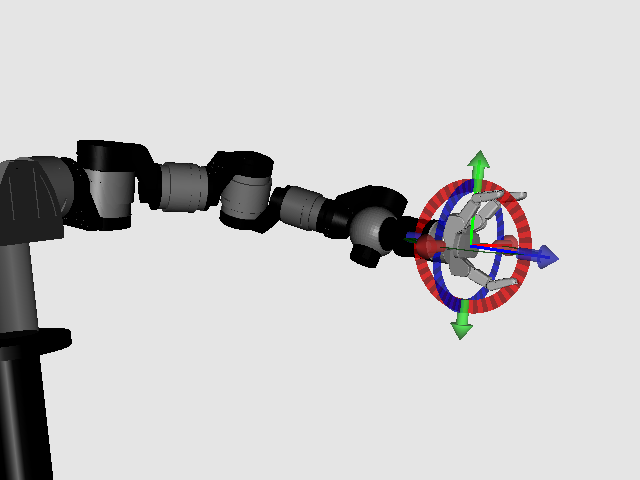
\includegraphics[width=0.48\textwidth]{fig/ik1.png}}
  \subfigure[][\label{fig:ik2}Flat feet constraint]{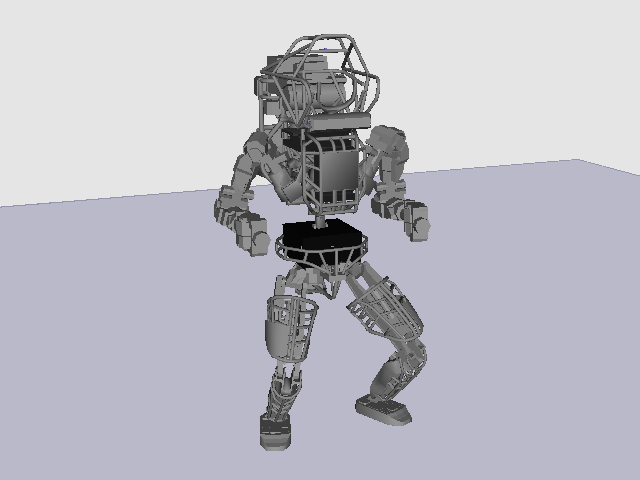
\includegraphics[width=0.48\textwidth]{fig/ik2.png}}
  \subfigure[][\label{fig:ik3}Sphere touching constraint]{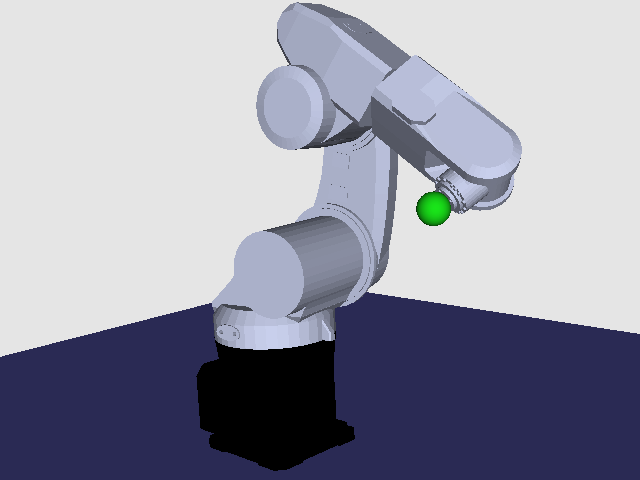
\includegraphics[width=0.48\textwidth]{fig/ik3.png}}
  \caption{Examples of various kinematic constraints}
  \label{fig:ik}
\end{figure}

Similar to the Gradient Methods mentioned above, KIDO allows the user to create and swap in any custom Error Method that they would like to. KIDO comes prepackaged with a Task Space Region\cite{Berenson_2011_6867} error method and will use that method by default. All of the constraints seen in figure \ref{fig:ik} can be achieved by adjusting the parameters of the \textbf{IK::TaskSpaceRegion} class in the following way:

\begin{tabular}{| l | c |}
  \hline
  \multirow{2}{*}{Figure \ref{fig:ik1}} & \multirow{2}{*}{Default Settings}              \\
                                        &                                                \\ \hline
  \multirow{2}{*}{Figure \ref{fig:ik2}} & Linear Bounds: ($\pm$Inf, $\pm$Inf, 0)         \\
                                        & Angular Bounds: (0, 0, $\pm$Inf)               \\ \hline
  \multirow{3}{*}{Figure \ref{fig:ik3}} & Linear Bounds: (0, 0, 0)                       \\
                                        & Angular Bounds: ($\pm$Inf, $\pm$Inf, $\pm$Inf) \\
                                        & [Offset the \textbf{EndEffector} from the surface of the body]     \\ \hline
\end{tabular}

An explanation of how to create your own custom \textbf{ErrorMethod} implementation is available at the end of section \ref{sec:ik_basic_framework}.

\subsubsection{Target}

With KIDO, we can take advantage of the frame semantics discussed in section \ref{sec:FrameSemantics} to conveniently express kinematic constraints in terms of arbitrary reference frames. Furthermore, due to the automatic updating discussed later in section \ref{sec:lazy}, the constraint will automatically adjust whenever its reference frame moves.

To achieve this, we have a target frame which acts as a reference frame for the parameters of the \textbf{ErrorMethod}. For the \textbf{TaskSpaceRegion} implementation of the \textbf{ErrorMethod}, the linear bounds will be evaluated relative to the origin of the target frame, and the angular bounds will be evaluated relative to the orientation of the target frame. In general, it is at the discretion of the implementer to decide how a custom implementation of an \textbf{ErrorMethod} utilizes the target frame, but the KIDO developers strongly urge users to implement their \textbf{ErrorMethod}s such that they use the target frame in an intuitive way. For example, if the goal of an \textbf{ErrorMethod} is to constrain the body to a parabolic surface, then the origin and orientation of the parabolic surface should be determined by the target frame.

A \textbf{SimpleFrame}, described in section \ref{sec:SimpleFrame}, is used as the target frame in the \textbf{InverseKinematics} framework. The target \textbf{SimpleFrame} can be  switched out for a different \textbf{SimpleFrame} (or a derivative class of SimpleFrame) at any time, but it cannot be switched out for any other type of \textbf{Frame}. In order to use an arbitrary \textbf{Frame} instance as the target frame for your kinematic constraints, all you have to do is set that \textbf{Frame} to be the parent of your existing target \textbf{SimpleFrame}, and then set the relative transform of your existing target \textbf{SimpleFrame} to an identity matrix. This design makes it extremely straightforward to express your target in whatever way is most convenient for your application.

\subsubsection{Objective Functions}

In KIDO, we treat Inverse Kinematics as an optimization problem. The \textbf{ErrorMethod} from section \ref{sec:ErrorMethod} describes a kinematic constraint for the optimization problem. The \textbf{GradientMethod} from section \ref{sec:GradientMethod} computes (an estimate of) the gradient of that constraint. In this section, we discuss the Objective \textbf{Function}, which describes a cost function which should be minimized while satisfying the constraints.

\begin{figure}
  \centering
  \subfigure[][\label{fig:red_ik1}Standing Tall]{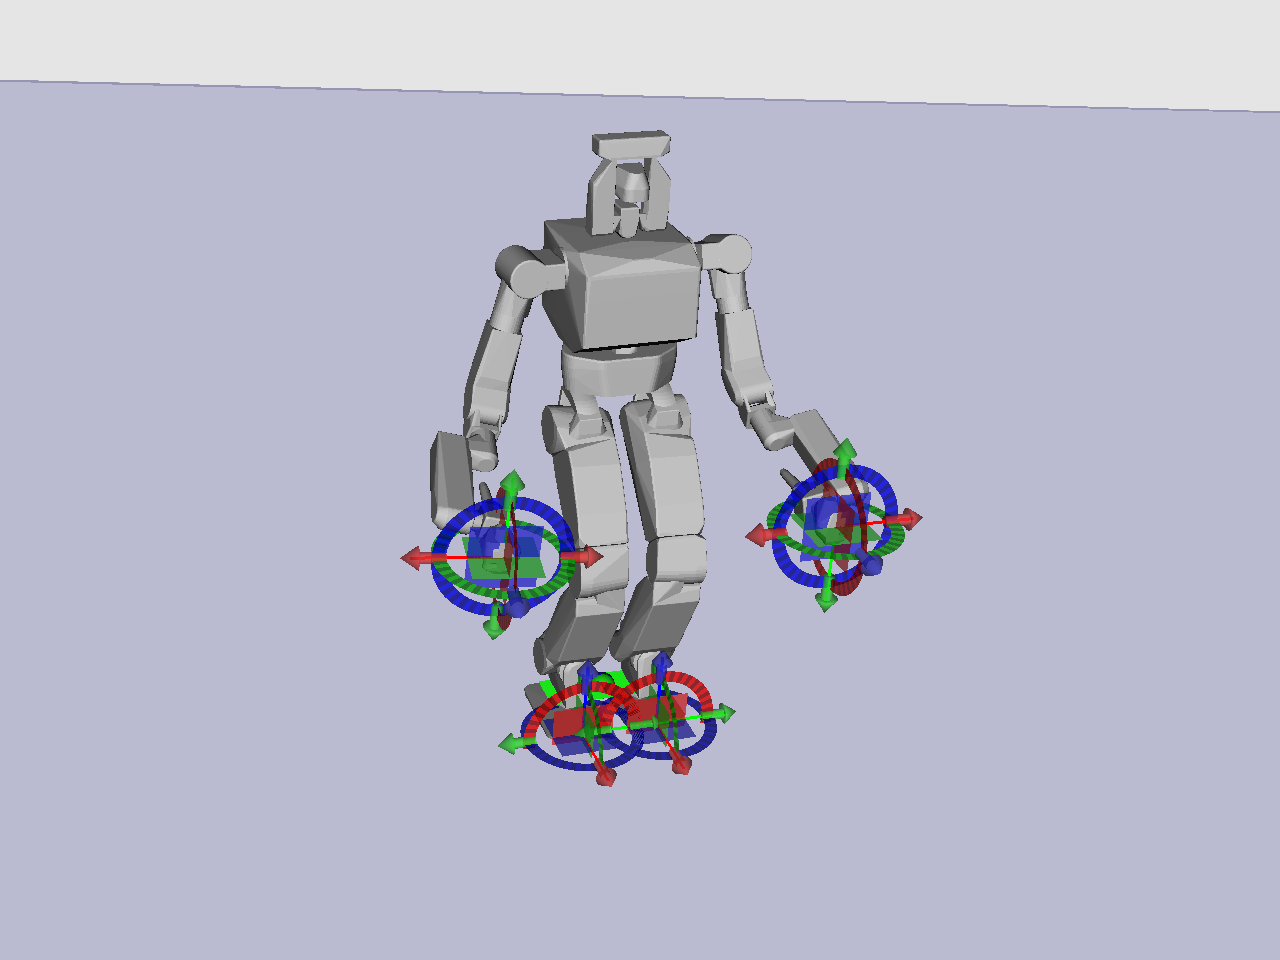
\includegraphics[width=0.48\textwidth]{fig/redundant_ik1.png}}
  \subfigure[][\label{fig:red_ik2}Squatting]{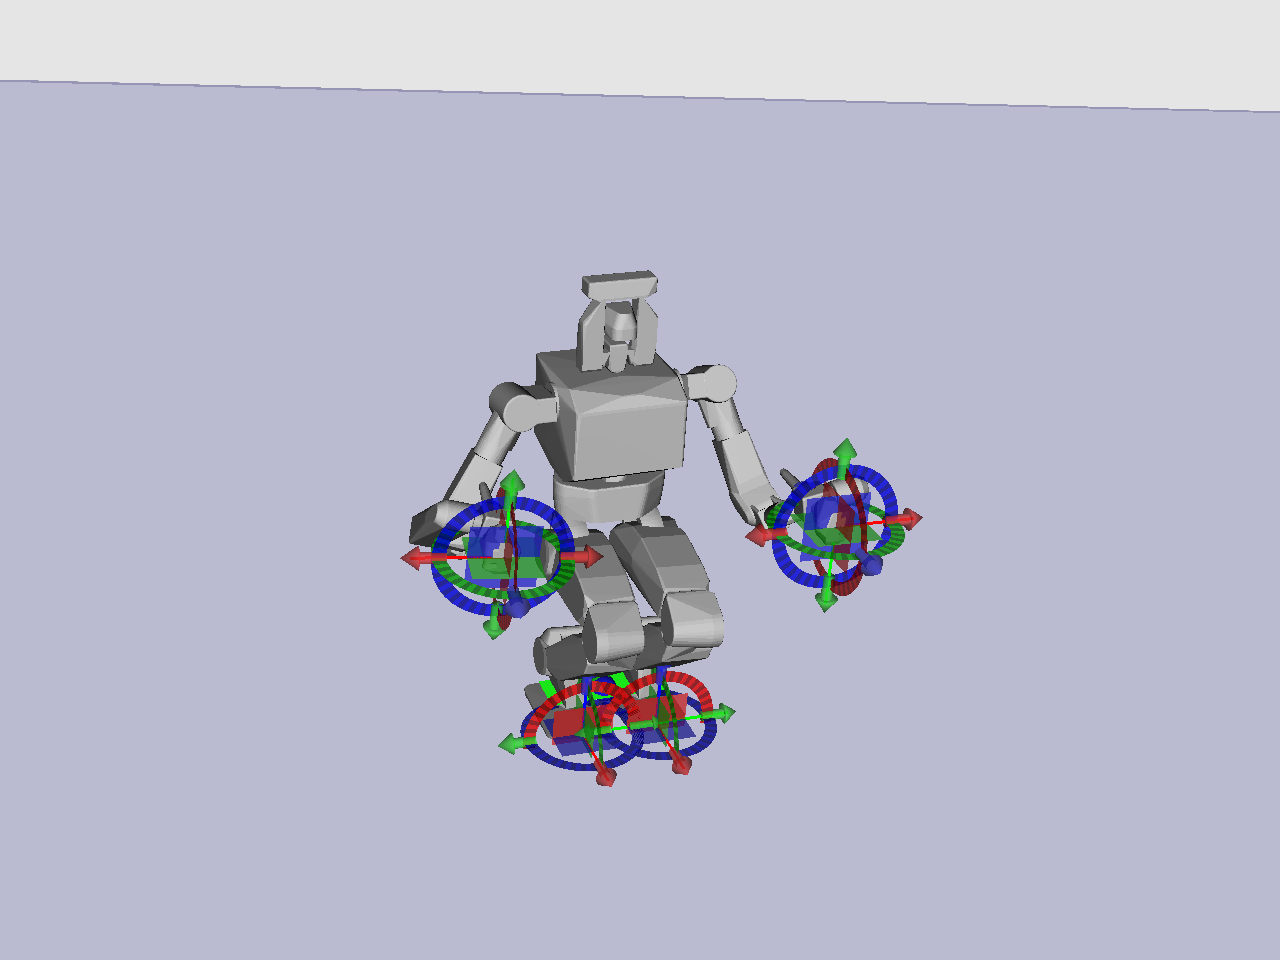
\includegraphics[width=0.48\textwidth]{fig/redundant_ik2.png}}
  \subfigure[][\label{fig:red_ik3}Leaning to the Right]{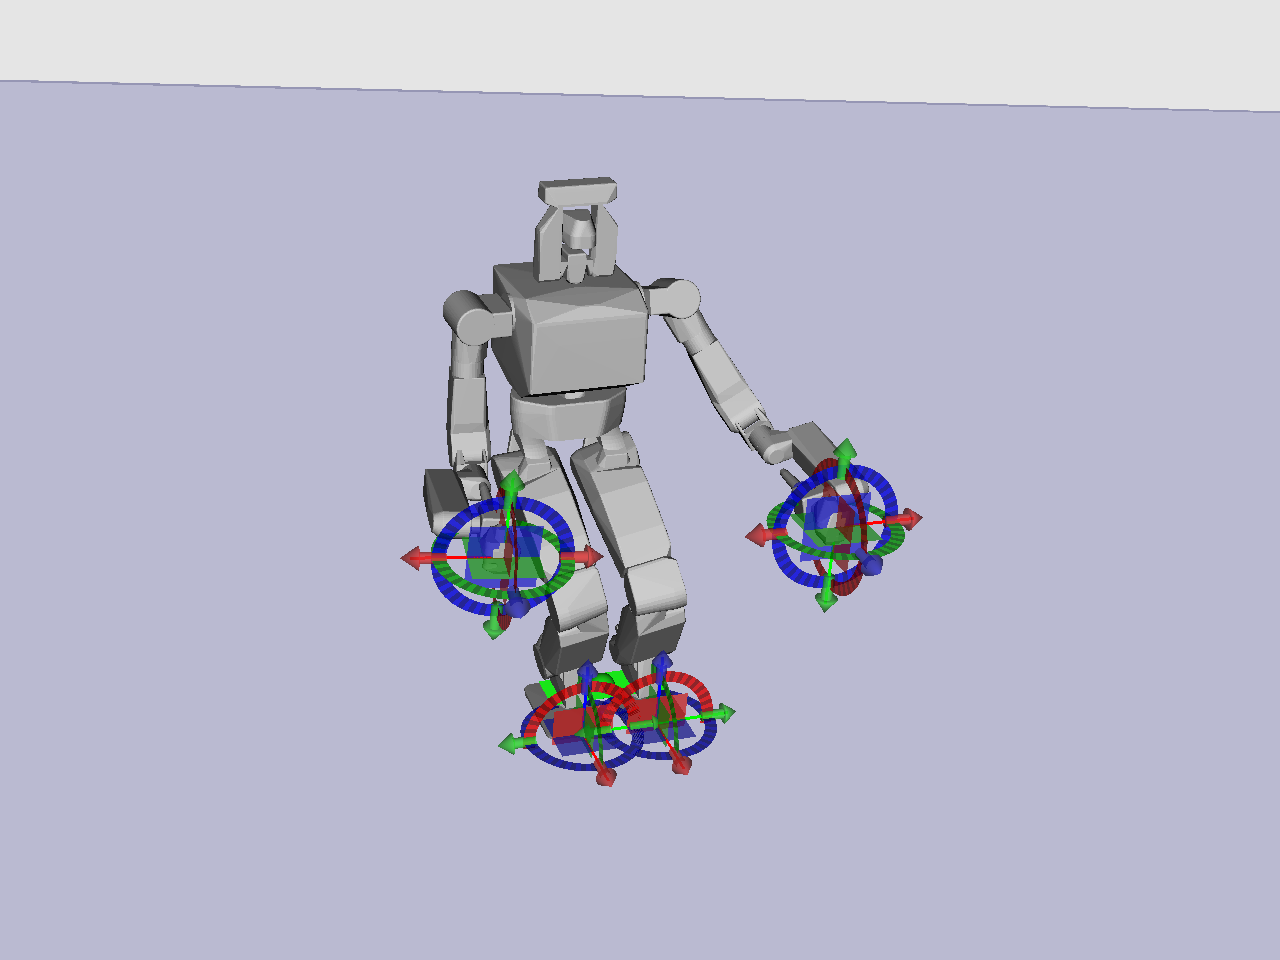
\includegraphics[width=0.48\textwidth]{fig/redundant_ik3.png}}
  \subfigure[][\label{fig:red_ik4}Leaning to the Left]{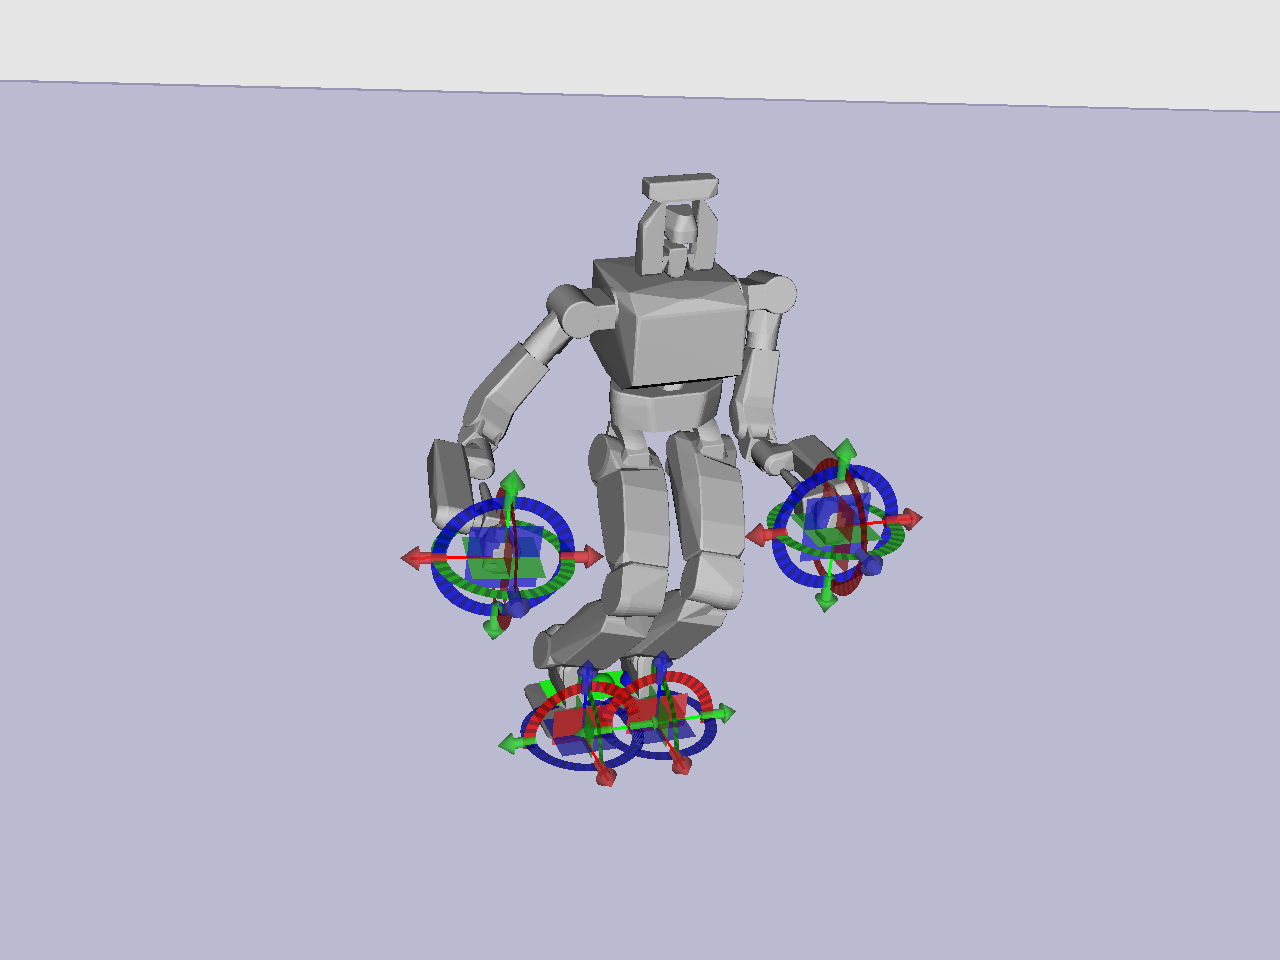
\includegraphics[width=0.48\textwidth]{fig/redundant_ik4.png}}
  \caption{Examples of kinematic redundancy. The kinematic constraints for all four panels are identical.}
  \label{fig:red_ik}
\end{figure}

By default, there is no objective function. As soon as a solution within the constraints is found, the result is returned. For kinematic structures with many redundant degrees of freedom, there may be infinite solutions to a given set of kinematic constraints, and some of those solutions might be more ``favorable'' than others. For example, in figure \ref{fig:red_ik} all four panels have the same exact kinematic constraints, but all four configurations are noticeably different. Depending on the context, this might or might not matter, but in some cases, there may be some valid configurations which are considered preferable to other valid configurations. In those cases, an Objective \textbf{Function} can be provided which will direct the solver towards a preferable configuration. The solver will seek to \textbf{minimize} the Objective Function, therefore it should be thought of as a \textbf{cost} function.

When performing inverse kinematics on a live robot, it might be crucial for all the robot's motions to satisfy the kinematic constraints, or else the task may fail. A common method for ensuring this is to project the objective through the null space of the constraint Jacobian. KIDO allows you to specify both an Objective function and a Null Space Objective function. The output of the Null Space Objective function will automatically be projected through the null space of the body's Jacobian, and then added to the overall Objective. If keeping the kinematic constraint satisfied is far more important than minimizing some objective, then that objective should be set as the null space objective and not set as the normal objective.

\subsubsection{Basic Framework}
\label{sec:ik_basic_framework}
The components that are mentioned in the previous sections are ultimately tied together by the framework of the \textbf{dynamics::InverseKinematics} class. The information flow within the framework can be seen in figure \ref{fig:ik_basic_framework}. \textbf{InverseKinematics} takes advantage of KIDO's \textbf{optimizer} framework, which is discussed in further detail in section \ref{sec:optimizer}.

\begin{figure}
\centering
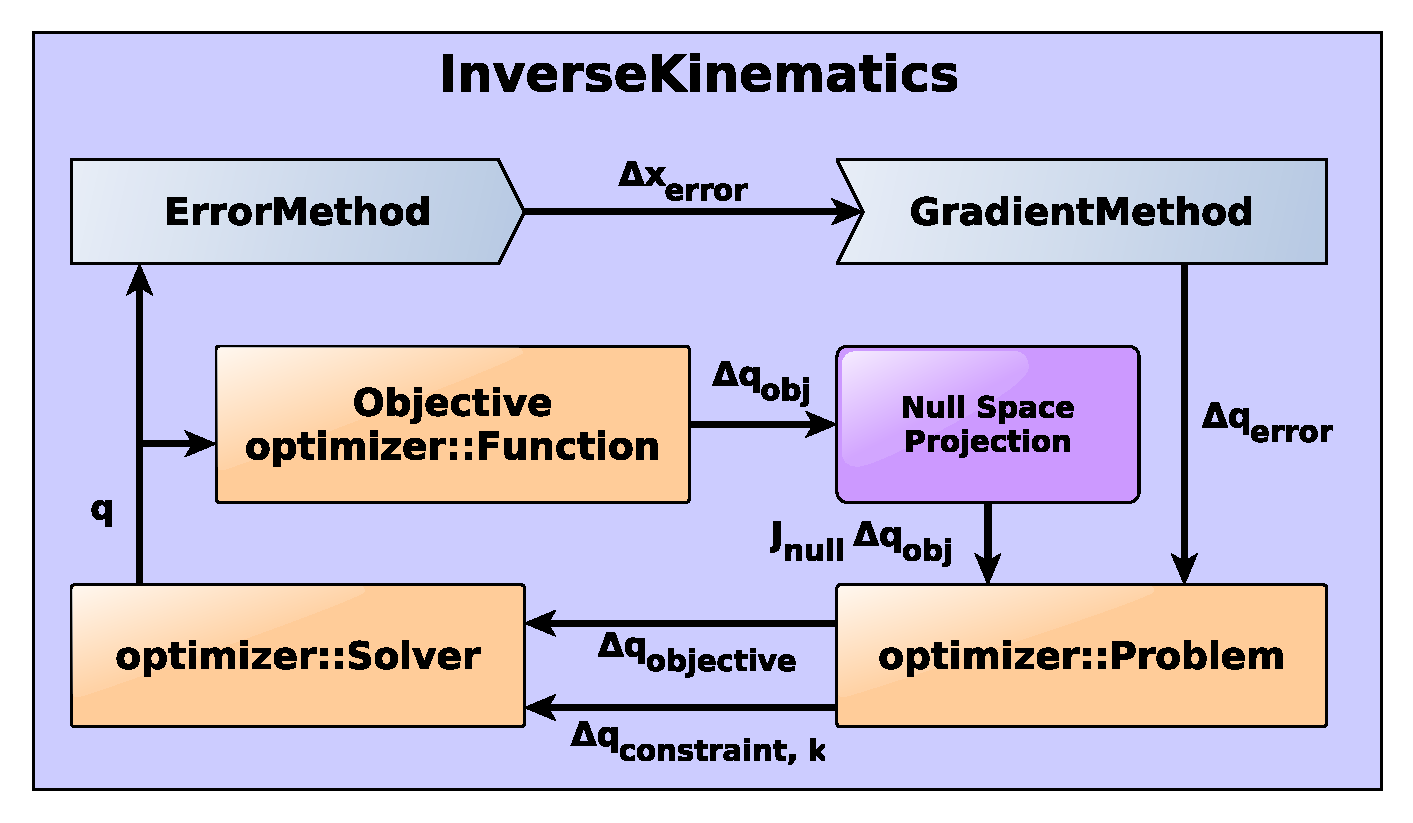
\includegraphics[width=\textwidth]{fig/ik_diagram.pdf}
\caption{Overview of \textbf{InverseKinematics} Framework}
\label{fig:ik_basic_framework}
\end{figure}

This entire framework is automatically constructed when an \textbf{InverseKinematics} object is created. Each piece has a default instantiation:

\begin{itemize}
  \item \textbf{ErrorMethod} is defaulted to a \textbf{TaskSpaceRegion} where each component of the linear and angular bounds are set to $\pm$\textbf{DefaultIKTolerance}, which is a small number (currently $1\times 10^{-6}$). The target frame is a \textbf{SimpleFrame} whose parent frame is \textbf{Frame::World()}, and whose world transform matches the current transformation of the body.
  \item \textbf{GradientMethod} is defaulted to the Damped Least Squares Pseudoinverse Jacobian method with a damping factor of \textbf{DefaultIKDLSCoefficient} (currently 0.05).
  \item \textbf{Objective} is a plain \textbf{optimizer::Function} which always returns zero. This is the same as not having an objective.
  \item \textbf{Null Space Objective} is also a zero function by default.
  \item \textbf{Problem} is automatically set up to contain the kinematic constraint and an objective which merges together the normal objective function and the projected null space objective function. As the user, you have the freedom to overwrite any of this by manually replacing the objective function or adding/remove constraints of your own. If standard problem setup is insufficient for your needs, this is where you have the freedom to completely reconfigure the problem. If the Problem is ever altered by the user, it can always be returned to its original setup by calling InverseKinematics::resetProblem().
  \item \textbf{Solver} defaults to KIDO's built-in \textbf{optimizer::GradientDescentSolver}. This is a simple gradient descent solver which has no third-party dependencies. This can be swapped out for a more sophisticated solver at any time. For an explanation of the different solvers that are available, see section \ref{sec:optimizer}.
\end{itemize}

Any of the default components can be swapped out with alternatives at any time. Users can also create their own custom implementations of each component by inheriting the base class for each and overriding a few pure virtual functions, listed below:

%\begin{itemize}
%  \item \textbf{ErrorMethod}
%\end{itemize}
\paragraph{kido::dynamics::IK::ErrorMethod} \
\begin{lstlisting}
// Override this by creating a new instance of your class type and returning it in
// a unique_ptr. This allows IK setups to be easily replicated which could be 
// useful for spawning threads to parallelize your computations.
//
// Note that the constructor of your class is required to take in an 
// InverseKinematics pointer as its first argument.
std::unique_ptr<ErrorMethod> clone(InverseKinematics* newIK) const;

// Override this by computing a 6D error vector. The first three components of the
// vector should represent orientation error (usually as Euler Angles or a logmap)
// and the last three components should represent translational error. NOTE THAT
// THIS IS THE REVERSE OF SOME CONVENTIONS. We do this in order to match 
// Featherstone's spatial vector convention, which is used in KIDO for spatial 
// velocity and spatial acceleration vectors.
Eigen::Vector6d computeError();

// We allow some flexibility in the exact meaning of the error vector that gets
// computed by computeError(), because iterative methods are robust to various
// representations of rotational error. However, Analytical methods typically
// require an exact desired transform. This function should construct an exact
// desired transform based on the current transform and the error (as computed
// by this error method) of the current transform.
Eigen::Isometry3d computeDesiredTransform(
    const Eigen::Isometry3d& currentTransform,
    const Eigen::Vector6d& error);
\end{lstlisting}

\paragraph{kido::dynamics::IK::GradientMethod} \
\begin{lstlisting}
// Override this by creating a new instance of your class type and returning it in
// a unique_ptr. This allows IK setups to be easily replicated which could be 
// useful for spawning threads to parallelize your computations.
//
// Note that the constructor of your class is required to take in an 
// InverseKinematics pointer as its first argument.
std::unique_ptr<GradientMethod> clone(InverseKinematics* newIK) const;

// This function should take in a 6D error vector (which will have been computed
// by the current ErrorMethod) and then modify the contents of the gradient 
// variable, which is passed in as an output parameter.
void computeGradient(
    const Eigen::Vector6d& error,
    Eigen::VectorXd& gradient);
\end{lstlisting}

\paragraph{kido::dynamics::IK::Analytical} is a specialized version of \textbf{GradientMethod} which allows users to plug in Analytical (a.k.a.\ Closed-Form) inverse kinematics solvers such that they are compatible with KIDO's inverse kinematics interface and hierarchical inverse kinematics solver (discussed in section \ref{sec:ik_hier_framework}). Note that computeGradient should not be implemented for an Analytical solver; that gets done automatically.

\begin{lstlisting}
// Override this by creating a new instance of your class type and returning it in
// a unique_ptr. This allows IK setups to be easily replicated which could be 
// useful for spawning threads to parallelize your computations.
//
// Note that the constructor of your class is required to take in an 
// InverseKinematics pointer as its first argument.
std::unique_ptr<GradientMethod> clone(InverseKinematics* newIK) const;

// This function should fill in the mSolutions protected variable and then return
// it. It would also be a good idea to call checkSolutionJointLimits() prior to
// returning, unless your function implementation checks the joint limits on its
// own.
//
// The Solution struct is a container which holds an Eigen::VectorXd for the
// configuration that's been generated, and a flag called mValidity which uses a
// bitwise map to indicate whether the configuration violates joint limits or is
// out of reach from the target transform. The expectation is that your 
// implementation will set mValidity to OUT_OF_REACH if the configuration does
// not reach the goal, and then you should call checkSolutionJointLimits() just
// before returning, which will inject LIMIT_VIOLATED into any Solutions whose
// joint limits are invalid.
const std::vector<Solution>& computeSolutions(
    const Eigen::Isometry3d& desiredTransform);

// An Analyical solver might only be able to solved for a subset of the degrees
// of freedom that are being utilized by an inverse kinematics solver. Because
// of this, you need to provide a function that indicates which degrees of
// freedom your Analytical method can provide solutions for.
//
// To determine how the remaining degrees of freedom get used, the Analytical
// class provides a setExtraDofUtilization(ExtraDofUtilization_t) function.
const std::vector<size_t>& getDofs() const;
\end{lstlisting}

It is also worth noting that the \textbf{Analytical} class has a \textbf{QualityComparison} function which is used to compare the qualities of various solutions. The default \textbf{QualityComparison} function will simply pick the configuration whose largest component of difference from the current configuration is the smallest. This is essentially the same as picking the configuration whose highest joint velocity would be the smallest out of all the options if the robot were to move to it from the current configuration. The chart below provides an example:

\begin{tabular}{| c | c | c || c | c | c | c | c |}
  \hline
  Rank & \textbf{Largest Component} & Norm  & $\Delta$q0 & $\Delta$q1 & $\Delta$q2 & $\Delta$q3 & $\Delta$q4 \\ \hline
  1    & 3.1                        & ~4.58 & 1.3 & 1.2          & 2.8 & 0.6          & \textbf{3.1} \\ \hline
  2    & 4.0                        & ~4.01 & 0.1 & 0.0          & 0.2 & \textbf{4.0} & 0.0          \\ \hline
  3    & 5.3                        & ~7.59 & 3.8 & \textbf{5.3} & 0.5 & 2.3          & 3.1          \\ \hline
\end{tabular}

The right side of the table shows the component-wise differences between the current configuration and each solution that has been generated. The left side shows the rank of each solution, along with the largest component of difference and the norm of its difference from the current configuration. Notice that the solutions are not sorted based on the norm; they are sorted in ascending order of the largest component in the difference vector. This sorting approach tends to reduce the likelihood of an ``elbow flip'' solution being selected.

\paragraph{kido::dynamics::IK::Function \& kido::optimizer::Function} are classes which should both be inherited when creating a class that represents an Objective Function. Technically, any class which inherits \textbf{optimizer::Function} can be used as an Objective Function, but it can only be cloned if it also inherits \textbf{dynamics::IK::Function}. Without that, the function will be replaced by a default zero-function in any clones that get produced.

\paragraph{kido::optimizer::Problem \& kido::optimizer::Solver} are standard tools from the kido-optimizer library, which is discussed in section \ref{sec:optimizer}.

\subsubsection{Hierarchical Framework}
\label{sec:ik_hier_framework}

The basic \textbf{InverseKinematics} framework is only designed to solve an inverse kinematics problem for a single body or end effector. This is typically sufficient for a simple robot arm, such as an industrial manipulator. More advanced robots or characters, such as humanoids, might require a more sophisticated type of inverse kinematics solver. In particular, they might need a solver that can solve for kinematic constraints on multiple bodies or end effectors simultaneously. To facilitate this, KIDO offers the \textbf{HierarchicalIK} class.

\begin{figure}
\centering
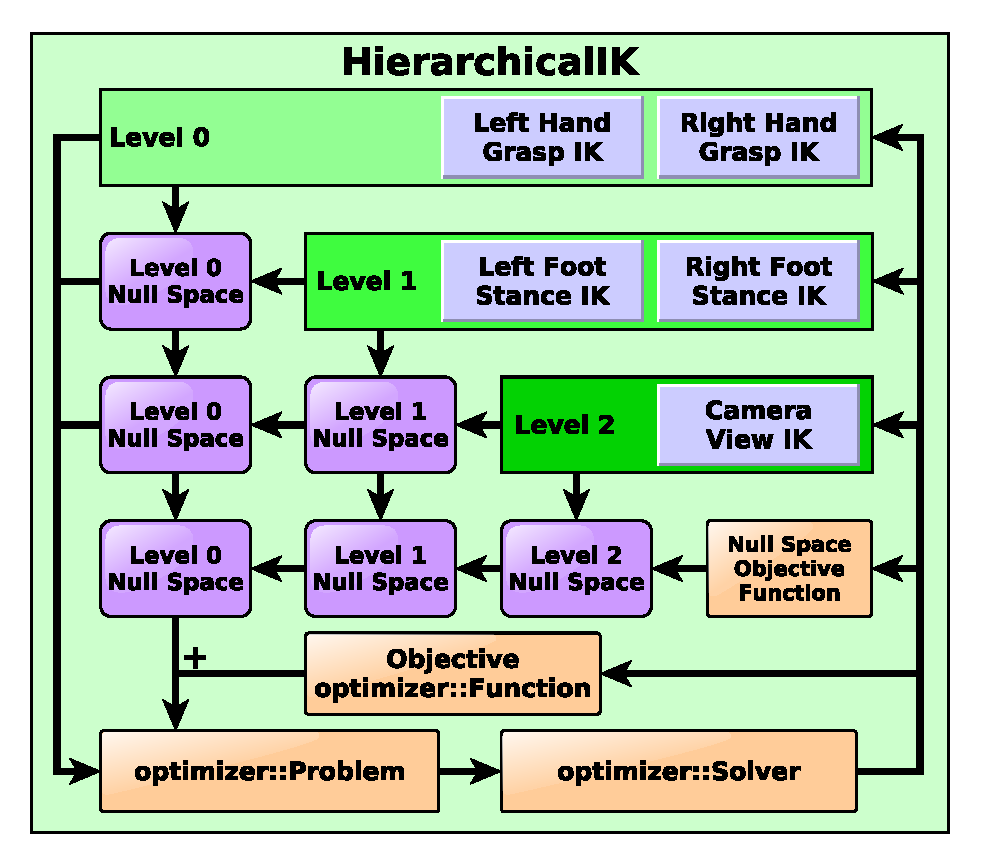
\includegraphics[width=\textwidth]{fig/hik_diagram.pdf}
\caption{Overview of \textbf{HierarchicalIK} Framework}
\label{fig:ik_hier_framework}
\end{figure}

Figure \ref{fig:ik_hier_framework} shows an example of how a \textbf{HierarchicalIK} object might be set up. Suppose we have a humanoid robot with two arms, two legs, and a camera on its head. We want the robot to grasp an object with both hands while standing in a balanced configuration, and we want it to look along a specific ray with its camera. The stance constraints on the feet are easily solved within the null space of the grasping constraints, so we place the IK solvers for the grasping constraints in level 0 (the highest priority level), and the stance constraints for the feet go below them in level 1. The camera view constraint is less important than any of the other four constraints, so we put that below all of them, in level 2.

The \textbf{HierarchicalIK} class can handle arbitrarily many hierarchy levels. All the inverse kinematics modules that are placed on the same level will be given the same amount of priority; their constraint functions will essentially be superimposed together. This superposition of constraint functions will then be projected through all the null spaces of any higher priority (lower level value) inverse kinematics modules. The level of an \textbf{InverseKinematics} object can be set using \texttt{InverseKinematics::setHierarchyLevel(size\_t)}.

Even though a Hierarchical object uses references to \textbf{InverseKinematics} objects, only the \textbf{ErrorMethod} and \textbf{GradientMethod} components of each \textbf{InverseKinematics} object gets used by a \textbf{HierarchicalIK}. This means that passing in an Objective or a Null Space Objective to the individual \textbf{InverseKinematics} objects will have no effect on a \textbf{HierarchicalIK}. Instead, the \textbf{HierarchicalIK} object has its own Objective and Null Space Objective. It also has its own \textbf{Problem} and \textbf{Solver}, so modifications to the \textbf{Problem}s and \textbf{Solver}s of the individual \textbf{InverseKinematics} objects also has no effect on a \textbf{HierarchicalIK} object. However, configuring an \textbf{InverseKinematics} module to use a specific \textbf{Analytical} (or any other \textbf{GradientMethod}) type \textit{will} have an impact on any \textbf{HierarchicalIK} object that it gets passed to. This allows \textbf{HierarchicalIK}s to string together multiple \textbf{Analytical} IK solutions simultaneously. For example, if a humanoid has an analytical IK solution for each limb, then the \textbf{HierarchicalIK} may be able to solve an arbitrary whole body inverse kinematics problem with a single iteration. Analytical IK solutions can also be seamlessly integrated with iterative solvers within a single \textbf{HierarchicalIK}. The \textbf{HierarchicalIK} will also respect whatever \textbf{ErrorMethod} is given to each \textbf{InverseKinematics} module.

The \textbf{HierarchicalIK} class is a pure virtual class, because it does not specify any way to decide which \textbf{InverseKinematics} modules it will use. Instead, there are two derived classes which offer different behavior:

\paragraph{CompositeIK} is a derivative of \textbf{HierarchicalIK} which allows the user to freely select which InverseKinematics modules it should utilize.

\paragraph{WholeBodyIK} is a derivative of \textbf{HierarchicalIK} which will automatically detect all \textbf{BodyNode} and \textbf{EndEffector} instances in a given \textbf{Skeleton} and use any \textbf{InverseKinematics} modules attached to them.